%Versuchsbeschreibung

In der Geoelektrik wurden drei verschiedene Messmethoden verwendet. Das ist die Wenner-Katierung, Schlumberger-Sondierung und die Tomographie. Sowohl die Wenner-Katierung als auch die Tomografie wurde über dem Basaltgang durchgeführt um diese Messmethode mit den übrigen vergleichen zu können. In Abbildung \ref{abb:PBasalt} sind die Profile der Wenner-Katierung und Tomografie abgebildet. Die Wenner-Kartierung wurde entlang E11-E12 durchgeführt, das Profil der Tomographie ist beschriftet. Zu sehen ist, dass das Profil der Geoelektrik über dem Profil der Magnetik und Gravimetrie liegt. Dadurch kann man direkt die Messergebnisse vergleichen und eventeull sehen welche Methode sich zum Untersuchen des Basalts eignet und welche nicht.\\
Die Schlumberger-Sondierung wurde auf dem gleichen Profil wie die Seismik-Messung mit Sissy durchgeführt, um die beiden Messungen vergleichen zu können. Dieses Profil ist das obere Profil E21-E22 in Abbildung \ref{abb:PWiese}.


%%%%%%%%%%%%%%%%%%%%%%%%%%%%%%%%%%%%%
\begin{figure}[h]
\centering
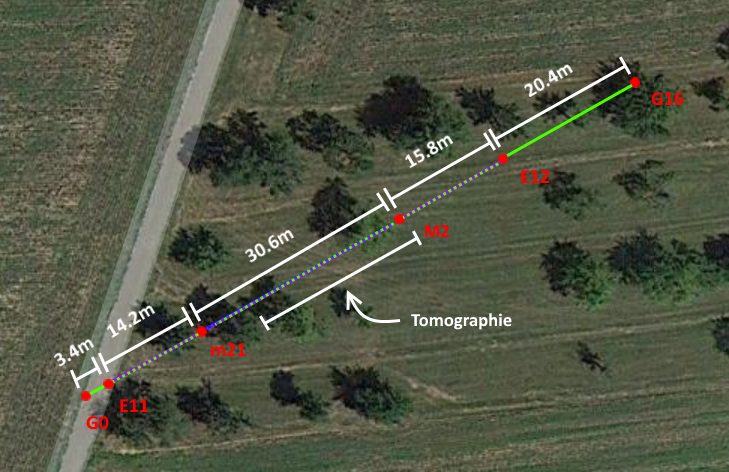
\includegraphics[width=0.6\textwidth]{fig/ElektrikMagnetikGravimetrie0gps.png}
\caption[Profile der Geoelektrik, Gravimetrie und Magnetik des Messgebiets am Basaltgang]{Profile der Geoelektrik, Gravimetrie und Magnetik des Messgebiets am Basaltgang. Die Graphik wurde von Rebekka Kirchgässner und Luisa Rank übernommen.}
\label{abb:PBasalt}
\end{figure}
%%%%%%%%%%%%%%%%%%%%%%%%%%%%%%%%%%%%

%%%%%%%%%%%%%%%%%%%%%%%%%%%%%%%%%%%%%
\begin{figure}[h]
\centering
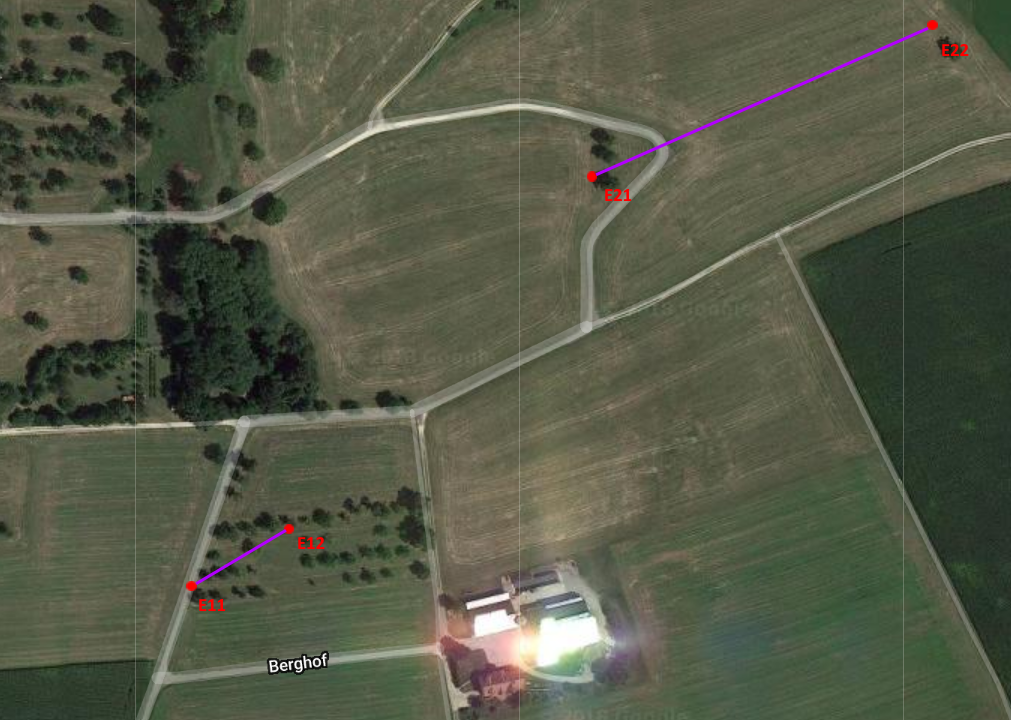
\includegraphics[width=0.6\textwidth]{fig/profilegps.PNG}
\caption[Profil E11-E12 und E21-E22 auf den beiden Messgebieten]{Profil E11-E12 und E21-E22 auf den beiden Messgebieten. Die Graphik wurde von Rebekka Kirchgässner und Luisa Rank übernommen.}
\label{abb:PWiese}
\end{figure}
%%%%%%%%%%%%%%%%%%%%%%%%%%%%%%%%%%%%
\newpage

\section{Wenner-Katierung}
Begonnen wurde mit der Wenner-Kartierung um die Lage des Basaltgangs genauer zu bestimmen. Damit wir die Tomografie möglichst genau über dem Gang durchführen
können. \\
Des weiteren soll eingeschätzt werden wie gut mit der diese Methode zum Vermessen des Basaltgangs geeignet ist.\\
\\
Die Kartierung wurde in einer Tiefe von 5 m vorgenommen. Dies ist begründet mit der Annahme, dass der Basaltgang vermutlich in ca. 1-2 m Tiefe beginnt und nach unten 
als unendlich angenommen werden kann. Je mehr Basalt im Bereich der Messung ist, desto größer ist die Auswirkung auf die Ergebnisse.\\
Die Anordnung ist orthogonal zum Basaltgang und wird auch orthogonal dazu verschoben. Orientiert wurde sich dabei an der Messung von Magnetik, es wurde 
entlang M2-M21 gemessen. Dabei wurde darauf geachtet, dass auch eine Messung komplett außerhalb 
des Einflussbereichs des Basalt liegt.\\
\\


 

\section{Tomographie}
Die Tomagraphie ist eine Kombination der ersten beiden Messmethoden. Die wurde auf dem gleichen Profil wie die Wenner-Kartierung durchgeführt.
Es wurden 48 Elektroden verwendet die, in einem Abstand von 50 cm, auf der gleichen Messlinie wie bei der Wenner-Kartierung aufgestellt waren. 
Die Mitte der Messlinie wurde auf einen Punk gesetzt, an dem auch die Mitte des Basaltgangs vermutet wurde. Insgesamt wurde also auf 24 m gemessen.\\
Als 0-Punkt für die Messung wurde das obere Ende des Messbands festgelegt.
Nachdem die Elektroden aufgestellt und angeschlossen wurden, wurde die Messung automatisch mit einem Messgerät automatisch ausgeführt. Auf das Ergebnis musste ca. 
eine Stunde gewartet werden.


\section{Schlumberger-Sondierung}
Sie Schlumberger-Sondierung wurde nicht auf dem Messgebiet über dem Basaltgang vorgenommen, sondern auf einer Wiese wesentlich weiter oben. Auf der Wiese 
bereits bei Seismik gemessen. Um unsere Ergebnisse von der Seismik-Messung und dieser Messung vergleichen zu können, wurde die Messung entlang der gleichen
Linie durchgeführt. \\
Da wir kein sehr großes geraden Gelände hatten und auch mit der Seismik ist keinen großen Tiefen gemessen wurde, betrug der Messbereich 200 m. Als Mitte 
haben wir den Punk des Mittelschusses der Hammer-Schlag-Methode (Seismik) verwendet.
In der Mitte des Profils haben wir angefangen die Elektroden zu Stecken. In beide Richtungen haben wir den Abstand exponentiell vergrößert. Die genauen Abstände kann man dem Messprotokoll dieser Messung im Anhang entnehmen.

